\chapter{Efficient Visual Annotation with Speech Recognition}
\label{ch:draw-and-tell}

``Sometimes, it is not who has the best algorithm wins, but who has the most data.". The importance of annotated training data has been proven many times in the history of computer vision. Taken object recognition as an example, the performance of algorithms leaped every time when a larger dataset was made available, from Caltech 101~\citep{FeiFei2004}, to Pascal VOC~\citep{pascal:2011}, to ImageNet~\citep{imagenet} and MSCOCO~\citep{coco:eccv}.  The tread may continue, but it is getting more difficulty as  annotations to an even larger scale are hardly affordable.  Developing efficient annotation approaches is one of the most effective solution to reduce the annotation cost.   In this chapter, we exploit the potential of speech recognition for visual object recognition, and propose a novel annotation approach which is 10x faster than standard ones for the task of semantic image segmentation. 

\section{Introduction}
Tremendous progress has been made during the last few years in 
object detection and semantic image segmentation due to (1) the success of
training deep convolutional neural networks (CNNs)~\citep{deepnet:nips12, decaf, vgg16} on large classification datasets and (2) the
flexibility of transferring CNN models pre-trained for image classification to the
task of object detection and semantic segmentation where not as much training data is
available~\citep{rcnn, Long_2015_CVPR, rcnn_crf}. Model transfer,
often called fine-tuning, partially lifts the strong need for large
training sets of CNNs. Yet, the fact remains that CNNs \emph{intrinsically} 
call for large-scale training data to unleash their learning capacity. 
As such, we can expect that the limit of CNNs for the tasks
is far from reached and that one of the obstacles 
is the cost of obtaining training samples.  
%a lack of large training datasets.
%  This follows the fact that pixel-wise segmentation masks are 
% enormously expensive to create. 

Obtaining training data for object detection or semantic image segmentation consists of two main
jobs: answering the \emph{what} and \emph{where} questions. \emph{What} is to annotate what
objects are present and \emph{where} is to indicate their locations in
the image.  As to \emph{what}, annotators usually need to choose class
names from some form of menus with the mouse and/or
keyboard~\citep{open:surface}. The procedure can be costly especially
when the number of classes considered is large. Imagine the amount of
work for annotators to find the class name out of a list of hundreds
of names for every object they annotate, not even to mention
attributes, views, etc. In other systems~\citep{whatpoint, coco:eccv},
binary questions ask whether object classes are present, which is also
very expensive when the number of classes is large, though exploiting
the hierarchy of classes may reduce the
cost~\citep{scalable:annotation, coco:eccv}. As to \emph{where},
various forms of annotations have been used for training: from the
full segmentation masks~\citep{rcnn, rcnn_crf, crfasrnn}, over
bounding boxes~\citep{weak:seg:xu, BoxSup, ConsCNN} or just single
points~\citep{whatpoint}, to nothing spatial at all (image-level
annotation)~\citep{markov:topic, cnn:em}.  As can be seen in Figure \ref{./draw_and_tell/fig:1}, the more
specific the annotation, the more informative it is, but also the more
expensive to obtain. %See for examples.

\begin{figure} [tb]
$\begin{tabular}{ccccccc}
%\hspace{-1mm}
%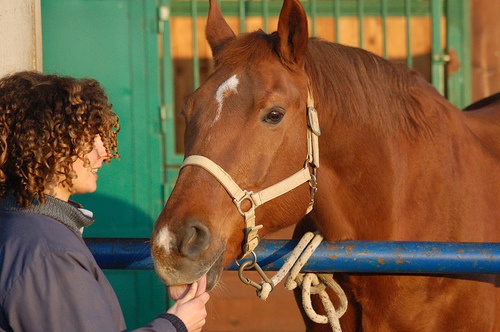
\includegraphics[width=0.15\linewidth]{./draw_and_tell/fig1/007109.jpg} &
\hspace{-2mm} 
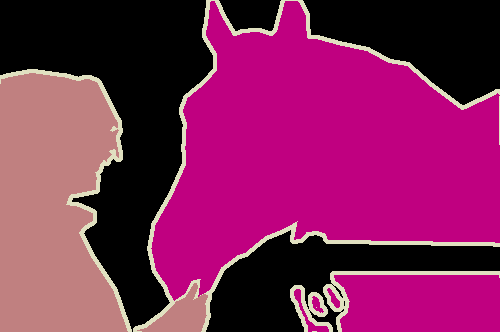
\includegraphics[width=0.18\linewidth]{./draw_and_tell/fig1/007109.png} &
\hspace{-4mm} 
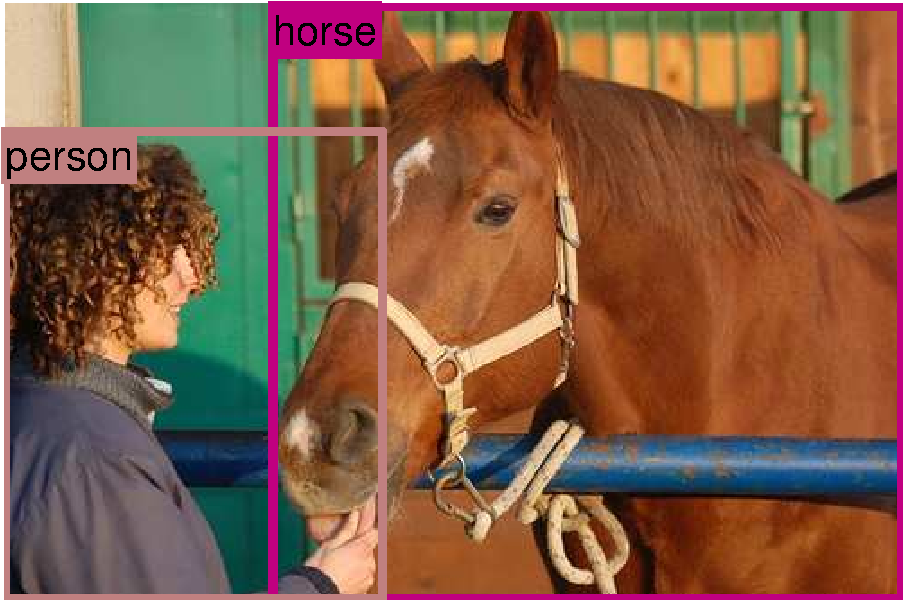
\includegraphics[width=0.18\linewidth]{./draw_and_tell/fig1/007109-bbx.pdf} &
\hspace{-4mm} 
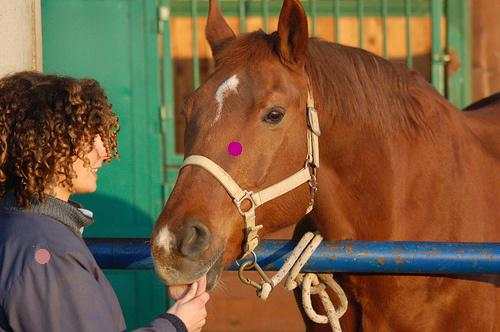
\includegraphics[width=0.18\linewidth]{./draw_and_tell/fig1/007109-point.jpg}&
\hspace{-4mm} 
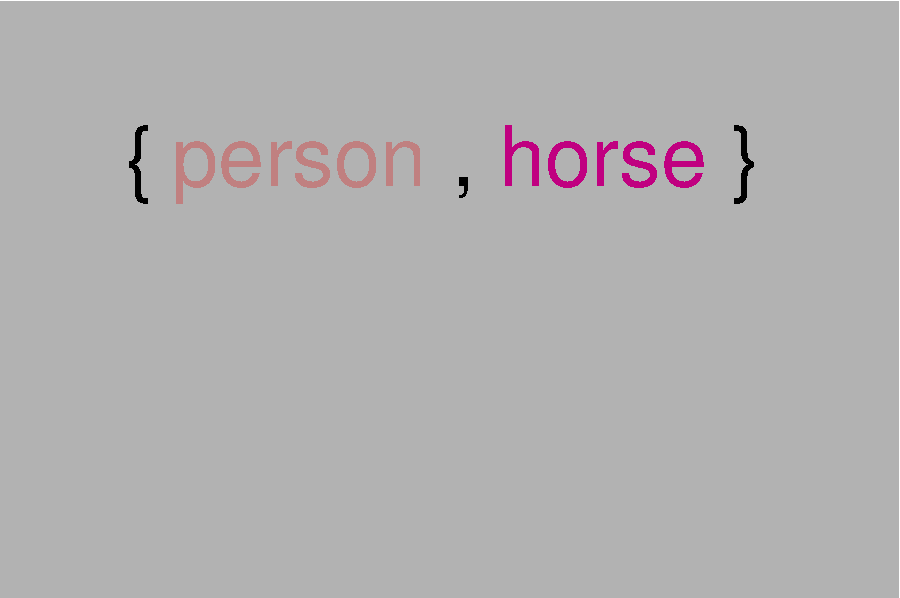
\includegraphics[width=0.18\linewidth]{./draw_and_tell/fig1/007109-keywords.pdf} &
\hspace{-4mm}
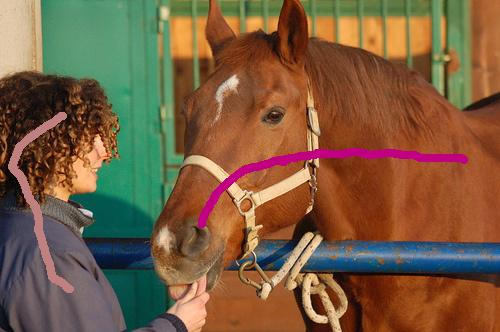
\includegraphics[width=0.18\linewidth]{./draw_and_tell/fig1/007109-scribble1.jpg} \\
%\footnotesize{\text{(a) image }} & 
\hspace{-2mm} 
\footnotesize{\text{(a) mask [\imouse]}} & 
\hspace{-2mm} 
\footnotesize{\text{(b) b-boxe [\imouse]}} &
\hspace{-4mm} \footnotesize{\text{(c) point 
[\imouse]}} & 
\hspace{-4mm} \footnotesize{\text{ (d) keyword
[\imouse]}} & 
\hspace{-4mm} \footnotesize{\text{ \textbf{(e) 
scribble} [\imouse+\iphone]}}  \\
\end{tabular}$
\caption{A comparison of our annotation (e) to other forms of
  annotations for semantic segmentation, ranging from (a) full
  segmentation masks, to (b) bounding boxes, to (c) single points, and
  to (d) image-level keywords. The devices to obtain these
  annotations are shown as well: others only use the mouse (+keyboard),
  while ours also uses voice input through a microphone.  }
\label{./draw_and_tell/fig:1} 
\end{figure}

In this work , we present a novel annotation method, which strikes a
balance between annotation cost and informativeness provided. In
particular, annotators are asked to draw scribbles (strokes) on objects of
interest, while saying aloud their class names (attribute if necessary). The 
scribbles are recorded to solve the \emph{where}
problem; the speech is recognized by a specially trained
recognition engine to solve the \emph{what} problem. 
In order to further increase the recognition accuracy of the scribbles 
(associating to object names), we integrate the speech recognition with a webly-supervised object recognition.  
The object recognition system is trained with images retrieved from image searching engine directly, and is applied to the image region where the scribble is drawn.  
An example of the annotation by our method is shown in Figure~\ref{./draw_and_tell/fig:1}, along with
that of other methods.

The method is inspired by two observations: (i) \emph{what} and
\emph{where} are handled separately in previous methods. For instance,
in~\citep{open:surface} annotators first mask out a region and then
assign a label to it; and in~\citep{coco:eccv} annotators
label the presence of objects in the first round, followed by positioning
them in the second round. This separation is unnecessary and
introduces extra cost, because the two problems are interdependent and
solved together by the annotators’ vision. It seems the separation is due
to the fact that only a single mode of input devices was used in the
previous methods, which is the mouse (+keyboard). We lift this
restriction by including the speech channel, which allows annotators
to communicate with the computer more naturally and efficiently. 
(ii) Drawing scribbles is another natural and efficient ability, and
has been widely used for interactive image segmentation. But to the best 
of our knowledge, it has not been applied to create training data for 
semantic image segmentation. We demonstrate that combining drawing and 
speaking can tackle both the \emph{what} and \emph{where} problems, 
leading to an efficient annotation method for semantic image segmentation.
We call the method \textbf{Draw\&Tell}.  


% annotate only one class each time, and the process loops over all
% classes of interest. This is inefficient because the because one image
% usually only contains very few (say 0~5) classes.  \textbf{check coco
%   how they annotate images}

% For each category found, the individual instances
% were labeled, verified, and finally segmented. Given the inherent ambiguity of
% labeling, each of these stages has numerous tradeoffs that we explored in detail.

% unprecedented number of images 
% for category detection, instance spotting and instance segmentation

%Having obtained the annotations, we convert them to heatmaps of the
%corresponding classes by combining interactive image segmentation
%(IIS)~\citep{geodesic:star} and ensemble clustering~\citep{dai:ensemble:eccv12}. 
%In particular, each scribble (i.e. stroke) on an object is taken 
%as the foreground object scribble in IIS, and the scribbles on other 
%objects belonging to the background. Scribbles for the background 
%are augmented by another set of scribbles sampled from the complete 
%background to avoid heavy bias to annotated objects. 
%The augmentation is done by randomly sampling scribbles
%from areas which are far apart from the foreground scribbles. 
%and are highly unlikely to be objects (reflected by objectness measures).
%Applying an IIS method using the scribbles generates a mask for the 
%object considered. To further increase robustness, we follow the idea of  ensemble clustering~\citep{dai:ensemble:eccv12} to run the IIS method multiple times with different
%augmented scribbles as constraints. The resultant object masks are then averaged to get the final heatmap of the object considered. The process is repeated for all object classes in the image, and the heatmaps  for classes not present are set to zero.

Having obtained the annotations, we convert them to soft confidence
maps of the corresponding classes by combining interactive image
segmentation and ensemble learning. We call these soft confidence maps semantic heatmaps.
Finally, we extend the standard CNNs model~\citep{Long_2015_CVPR} to
accommodate the soft semantic heatmaps as training data rather than the
standard crisp labels.  The pipeline of the method is shown in
Figure \ref{./draw_and_tell/fig:2} (right hand side), which also shows the standard fully
convolutional network~\citep{Long_2015_CVPR} for ease of comparison. We
show in experiments (i) that our annotation method is $11$ times faster than
pixel-wise annotation, and also faster than
conventional image-level annotation; (ii) that our adapted CNNs trained with the
annotations yields significantly better results than the CNNs trained
with image-level training data, and yields results comparable with
those of the CNNs trained with pixel-wise annotations; and (iii) that under the same annotation budget, our annotations, combined with our learning method, yield better results than the conventional precise annotations.
 
 \begin{figure*}[!tb]
\centering
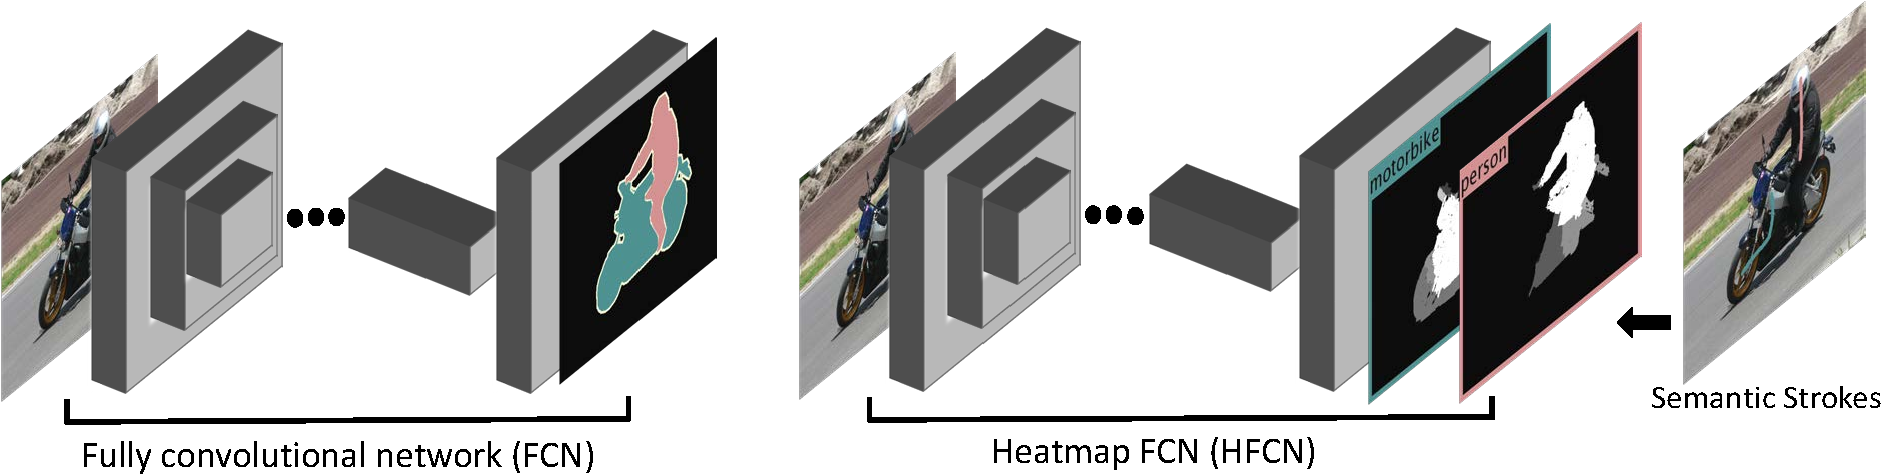
\includegraphics[width=0.95\linewidth]{./draw_and_tell/fig2/figure2-crop.pdf}
\caption{The framework of the standard fully convolutional network
  (FCN)~\citep{Long_2015_CVPR} and our heatmap-based FCN.}
\label{./draw_and_tell/fig:2} \vspace{-3mm}
\end{figure*}

Our contributions are mainly: (i) a new method which combines webly-supervised vision and automatic speech recognition to efficiently create training data for semantic image segmentation,
and (ii) a method to train CNNs with scribble-based training data, by converting scribbles to soft heatmaps and extending the standard neural networks. 
Introducing speech recognition into visual annotation is novel and 
our method can be used for other vision tasks as well, such as annotations for object detection, part detection, attribute detection and view estimation. The integration of webly-supervised object recognition and speech recognition can also serve as an example of combing vision and speech. 

This chapter is organized as follows. Section~\ref{drawtell:sec:related} presents
related work. Section~\ref{drawtell:sec:annotation} details the
annotation method, followed by Section~\ref{drawtell:sec:method} which is devoted
to the segmentation method. Section~\ref{drawtell:sec:experiments} then reports on the
experiments and Section~\ref{drawtell:sec:con} concludes the paper.


\section{Related Work}
\label{drawtell:sec:related}

Previous work related to ours mainly falls into two groups:
semantic image segmentation and integration of
vision and language (speech).

\subsection{Semantic Image Segmentation}
\textbf{Methods:} There is a rich literature of semantic image
segmentation (SIS)~\citep{texton:boost, fully-crf}, and the field has
made tremendous progress since CNNs were applied. The seminal
R-CNN~\citep{rcnn} and the follow-up systems~\citep{Long_2015_CVPR,
  rcnn_crf, crfasrnn} yield significantly better performance than
previous methods. As noted above, SIS through CNNs has probably not come
to full fruition yet due to the small size of the existing training
sets. Several successful attempts have been made to use weaker
supervision in order to reduce the annotation cost.  For instance,
\citep{cnn:mil} exploits multiple instance learning to train
FCN~\citep{Long_2015_CVPR} with image-level annotations. \citep{cnn:em,
  BoxSup, ConsCNN} leverage the power of object proposals to train FCN
with object bounding-boxes. \citep{whatpoint} presents a system to
train FCN with point annotation -- objects are indicated by single
points.  In the same vein our work tries to train FCN with annotations
that are efficient to obtain. 

%various forms of weak supervision ~\citep{weak:seg:xu}
\noindent
\textbf{Supervision:} Datasets play a critical role in computer
vision. They qualitatively `define' the learning tasks and guide
research directions.
% , which has been proved in many fields, such as
% optical flow~\citep{flow:dataset} and image recognition~\citep{imagenet,
%   pascal:2011}. 
Training annotations for SIS often come as full segmentation masks
(c.f. Figure \ref{./draw_and_tell/fig:1}). The most popular ones fall into this
category: CamVid~\citep{camvid:data} for outdoor scenes,
NYU~\citep{NYU} for indoor scenes, PASCAL~\citep{pascal:2011} and
COCO~\citep{coco:eccv} for general objects, and
PASCAL-Context~\citep{pascal:context} for objects in context.  Creating
datasets for SIS is very expensive even with excellent annotation
tools~\citep{open:surface, label:me}. As a result, methods were
proposed to reduce the cost.  For instance, \citep{scalable:annotation,
  coco:eccv} exploit the hierarchical structures of object classes to
reduce annotation space. \citep{AFrameSel, expected:loss} exploit
active learning techniques to suggest the most informative samples to
annotate under a budget. \citep{detect:eyetr} employs eye tracking
systems to help create training data for object detection.  Our
proposal is to exploit speech recognition to help dataset creation for
SIS.

% There are methods to transfer knowledge learned from datasets of
% relevant tasks to the task of which the annotations are scarce.  For
% example, \citep{lsda} transfers the the CNN models learned for
% classification to object detection, and \citep{SuTransfer} transfers
% the supervision of annotated RGB images to other data modalities such
% as depth and flow. Crowd-sourcing has been widely used in the field as
% well and it is complementary to all the techniques mentioned above.



% \citep{human:in:loop} provides a hybrid
% human-computer algorithm for object recognition by putting a human in
% the loop to help computers.  

% segmentation masks ~\citep{open:surface, label:me, camvid:data}
% bounding box \citep{imagenet, pascal:2011}
% point \citep{whatpoint}
% semantic object selection~\citep{object:selection}

% \textbf{crornd sourcing}
% Beat the MTurkers~\citep{beat:AMT}
% other source of input: 

% The community has also created datasets containing object attributes
% [8], scene attributes [9], keypoints [10], and 3D scene information
% [11]. This leads us to the obvious question: what datasets will best
% continue our advance towards our ultimate goal of scene understanding?

\subsection{Integration of Vision and Language (Speech)}
Research interest in integrating vision and language has increased
recently, e.g. for image/video caption generation~\citep{ show:tell:caption, youtube2text,
  fgm:coling14, deep:alignment:vl, babytalk}.  The objective is to
learn from a corpus of sentences and images / video snippets to
generate meaningful descriptions for new images. One of the main
research topics is the alignment of representations from the two
different domains: vision and language. In terms of language\&vision
understanding, our goal is more conservative, because the words we
handle are restrictive and vision and language are aligned with human
help.  However, our purpose of the integration is different.
% LUC: THIS POINT IS NOT SO CONVINCING. PROBABLY AN ERROR LEFT OR RIGHT
% WOULD BE OF LIMITED INFLUENCE IN OUR CASE, AS THERE WILL BE MANY MORE
% EXAMPLES OF A CLASS,
% BUT IF ONE WANTS TO GENERATE A CAPTION FOR A SPECIFIC IMAGE, THERE IS 
% NOT MUCH ROOM FOR MISTAKES? 

Speech-driven interfaces are going through a renaissance, with popular
commercial products like Apple's Siri. The most relevant to our work
are those integrating speech and vision. Pixeltone~\citep{pixel:tone}
and Image spirit~\citep{image:spirit} are examples that use voice
commands to guide image processing and semantic segmentation. The
difference between image spirit and our work is that they use voice
commands to refine labeling results and we use them to collect
training data. Also, image spirit uses voice commands alone, while our
method combines speech input with mouse interactions. There also is
academic work~\citep{show:tell, speech:anno:img, speech:retri:img,
  video:anno:knowledgebase} and an app~\citep{smile} that use speech to
provide image descriptions.  Again, our purpose is very different.

%%%%%%%%%%%%%%%%%%%%%%%%%%%%%%%%%%%%%%%%%%%%%%%%%%%%%%%%%%%%%%%%%%%

\section{Speech-based Annotation}
\label{drawtell:sec:annotation}

\subsection{The Draw \& Tell Annotation Tool}

This section describes our annotation method, which consists of two 
parts: drawing scribbles on the objects and telling the system their 
names. Drawing scribbles is straightforward and we follow popular
interactive image segmentation (IIS) methods~\citep{geodesic:star} to
record the mouse tracks. As to the speech recognition, we draw on the state-of-the-art, end-to-end speech recognition systems~\citep{end-to-end:speech}, trained with bidirectional recurrent neural networks under the connectionist temporal classification loss function. The systems successfully avoid the significant human effort in creating the pronunciation dictionary. The characters are then decoded to words with a dictionary of desirable class names by the CTC Beam Search algorithm in~\citep{end-to-end:speech}. Improving such a system itself is challenging and beyond the scope of this paper, thus we choose to treat the system as a black box and operate on an n-best list of possible object names for each utterance. 

Speech recognition is a complex research area in its own right, and there are still problems  in recognizing natural speech with high accuracy~\citep{SR:review}. We, however, want to use it to simplify 
the task of annotation, for which high accuracy is required. Fortunately, some 
constraints can be imposed in our case, which our annotation task naturally 
fulfills. The constraints and solutions are:
\begin{itemize}
\item Constraining the vocabulary and syntax of the utterances to
  ensure robust speech recognition. For our annotation, the vocabulary
  is restricted to the names  of the objects of interest,
  and we can also instruct annotators to follow a specific syntax.

\item Synchronizing the speech input with mouse input. We instruct the annotator to only say the object names while they draw the scribble on the corresponding object, not at any other time. The speech recognition engine uses this synchronization to better identify speeches relevant to the object being annotated.

\item Re-ranking the n-best words by integrating information from visual object recognition, as analyzing the visual content in the drawing area provides complementary information. We choose to learn the recognizer in a webly-supervised manner, where images retrieved from image search engines such as Google and Bing are used directly for the training. This integration is also interesting in the wider context of combining vision and speech.  Section~\ref{drawtell:sec:web} elaborates the method. 

\end{itemize}

% \begin{figure*}[!tb]
% \centering
% %\includegraphics[width=0.95\linewidth]{./draw_and_tell/fig2/annotation.pdf}
% \framebox(200,300){}
% \caption{annotation interface and annotation examples.}
% \label{./draw_and_tell/fig:3}
% \end{figure*}
\begin{figure}[!tb]
\centering
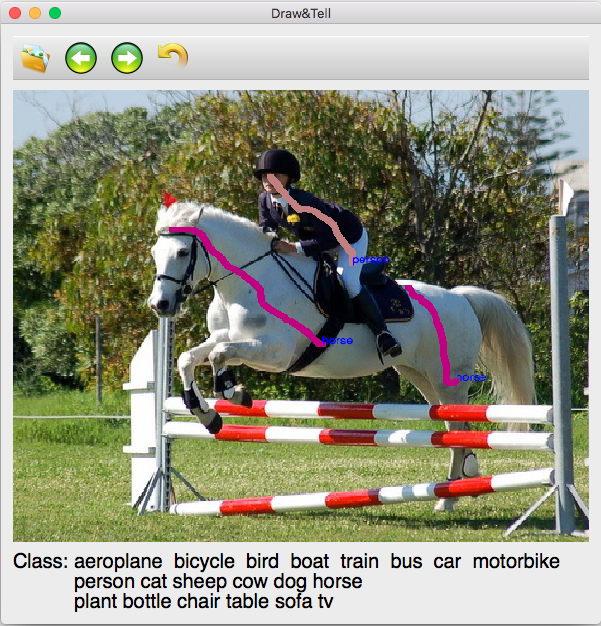
\includegraphics[width=0.8\linewidth]{./draw_and_tell/figSM/draw_tell_interface.png} 
\caption{The interface of Draw\&Tell.  Annotators can draw scribbles on objects of interest and speak their names in the meanwhile. The names of all the classes of interest are shown at the bottom for reference. The names of the object are obtained by speech recognition and are shown right after the drawing of the scribbles. Annotators can correct the result if it is wrong.}
\label{fig:drawtell:interface}
\end{figure}


As a fall-back solution, Draw\&Tell provides ways to permit correction of the recognition errors, by either repeating the operation (drawing + speaking) for the same object;
%   with the constraint that the new scribble overlaps with the one to be corrected (a new annotation
%   otherwise); 
or typing the object name directly.  The annotator will be asked to
review the name list if the system fails multiple times to recognize
the speech, mainly because the spoken words are out of the dictionary.  
Our implementation is built on top of the open source code of~\citep{lexfree2015}. 
The interface of Draw\&Tell is shown in Figure~\ref{fig:drawtell:interface}. 



\subsection{Integration with Webly Supervised Object Recognition}
\label{drawtell:sec:web}
As discussed in the previous section, speech recognition still has problem for high-precision applications like ours. Thus, we propose to re-rank the n-best words (object names) from the speech recognition engine by using visual information. The idea is straightforward as follows: once a scribble is drawn, a corresponding image region is cropped and fed into an object recognition system for visual recognition. The region is generated by choosing an object proposal out of $500$ candidates yielded by edge-box~\citep{edge:box}: (i) obtaining the enclosing bounding-box of the scribble, and (ii) choosing an object proposal with which the bounding-box has the highest intersection-over-union score. 
The recognition scores are then fused with the scores from speech recognition to obtain the name of the object.  %Figure \ref{./draw_and_tell/fig:fusion} for an example of the integration. 

The object recognition system can be trained with samples collected by conventional annotation methods, if available. We here explore the potential of training it with web images, due to (i) an enormous amount of visual data is online to use for free; and (ii) noisy  recognition (up to some level) is acceptable here as it is only used to complement speech recognition, which itself already performs well for a small dictionary of pre-defined words, though not perfect. 

We follow the footprint of~\citep{webly:cnn} to train a webly-supervised RCNN~\citep{rcnn} model for object recognition. Our RCNN is trained with a classification loss on images returned by Google directly -- images returned by the same keyword are taken as of the same class. The rationale is that the top images returned by Google mostly come with a clean background and a single centered object of the query class.  If needed, more sophisticated techniques can be used to prepare the training data, such as seeds-based co-segmentation~\citep{webly:cnn}.  In this work, we downloaded $2500$ images for each class, and fine-tuned the VGG Net~\citep{vgg16} pre-trained on ImageNet~\citep{imagenet}. The integration of speech recognition and webly-supervised object recognition is done by simply fusing their posterior probabilities: 
\begin{equation}
  P(y | \mathbf{v}, \mathbf{x}) = \sigma  P(y| \mathbf{v}) + (1-\sigma)  P(y|\mathbf{x})
\end{equation}
where $y \in \{1, ..., K \}$ denotes the object names with $K$ the number of classes, $\mathbf{v}$ the voice represented as spectrograms, $\mathbf{x}$ the cropped image region, and $\sigma$ a scalar value to balance the two terms. $\sigma$ is set to $0.7$ empirically in this work to put more weight on speech recognition as the object recognizer is trained with noisy data.      
 
% We address the complete LVCSR problem. Our system trains on utterances which are labeled by word-level transcriptions and contain no indication of when words occur within an utterance.


% For implementation, we draw on use the state-of-the-art speech
% recognition engine CMUSphinx~\citep{sphinx} and more specifically the
% PocketSphinx. We re-trained a new dictionary and language model for
% robust recognition, which specifically focuses on the object names of
% interest. Since our text corpus is small, compared to that for
% general speech recognition, the model can be trained by simply
% uploading the text corpus to CMUSphinx's web
% service~\citep{sphinx:webtrain}.

% , i.e. the $20$ class names of PASCAL
% VOC in our experiments. 
 
% LUC: THAT SOUNDS LIKE A MAJOR LIMITATION. 20 CLASSES IS A VERY LOW 
% NUMBER COMPARED TO WHAT CNN OBJECT DETECTION IS USED FOR THESE DAYS?
% AND WHAT DOES IT TAKE TO TRAIN FOR MORE / OTHER CLASSES. IS THAT REALLY
% EASY, ALSO FOR MANY CLASSES ? 


% LUC: THIS WOULD BE AN ISSUE IF FINE-GRAINED CLASSIFICATION IS THE TARGET.
% PUPPET AND DOG MAY IN SUCH CASE E.G. NOT BE CONSIDERED THE SAME ANY LONGER. 

% For the acoustic model, we use the one provided
% for US English. A new model can be trained for the annotators' accent
% for better performance if necessary.
% LUC: AGAIN, THIS SOUNDS LIKE BEING QUITE COMPLICATED. IT WOULD BE GOOD
% TO ADD SOME EXPLANATION THAT THIS IS QUITE EASY TO DO ALSO FOR PEOPLE
% WHO ARE NON-EXPERTS IN SPEECH? LIKE VISION RESEARCHERS. 

\subsection{Annotation Results}
Three results are reported: (i) recognition accuracy of object names,
(ii) annotation accuracy of the scribbles, and (iii) annotation speed
of our method.

\textbf{Recognition accuracy for object names}: Our method is
evaluated with a comparison to PocketSphinx~\footnote{Sphinx: \url{http://cmusphinx.sourceforge.net/}}, a standard
speech recognition engine. For fair comparison, we re-trained a new
dictionary and language model~\footnote{They are trained by simply
  uploading the text corpus to CMUSphinx's web
  service, available at url{http://www.speech.cs.cmu.edu/tools/lmtool-new.html}}.  for PocketSphinx as well so that
it focuses on the object names of interest.  The evaluation is
conducted on the box annotation of PASCAL VOC 2012~\citep{pascal:2011}
and that of MSCOCO dataset~\citep{coco:eccv}.  An annotated object in
the image is highlighted and its name is displayed. Annotators are
asked to draw scribbles on the object while speak aloud the name
displayed.  Examples are shown in the supplementary material.  The
recognition result will be compared to the ground truth and the
average accuracy is reported. $20$ object instances are sampled for
each object classes, leading to $400=20\times 20$ objects for PASCAL
VOC and $1760=20\times 88$ objects for MSCOCO. Three annotators
(graduate students) are asked to perform the annotation, and their
results are averaged. Table~\ref{table:class:eval} shows the results.

The results shows that our method performs significantly better than
the pure speech recognition methods, namely the HMM-GMM based method
PocketSphnix, and the bidirectional RNN based
method~\citep{end-to-end:speech,lexfree2015}. Webly-supervised object
recognition provides reasonably good results, but itself alone is
still not enough to be used for the annotation task. By combining the
strength of vision and speech, our method yields excellent results for
the $20$ classes of PASCAL VOC, and quite good results for the $88$
classes of MSCOCO. The results suggest that our method is accurate
enough to be used directly for annotation tasks of around $20$
classes. For more classes like that in MSCOCO, people often annotate
them in a hierarchical manner~\citep{coco:eccv}, leading to annotation
tasks with smaller number of classes, which makes our method
applicable as well.  In the rest of this work, we will mainly evaluate
our annotation method on the $20$ classes of PASCAL VOC.

\begin{table}[tb]
  \centering
  \setlength\tabcolsep{1mm}
\begin{tabular}{|c|c|c|c|c|c|c|c|c|c|  }
 \hline
 \multicolumn{4}{|c|}{PASCAL VOC} &  \multicolumn{4}{c|}{MSCOCO} \\
 \hline
 \multirow{2}{*}{PocketSphnix} &  \multicolumn{3}{c|}{Ours} &  \multirow{2}{*}{PocketSphnix} &  \multicolumn{3}{c|}{Ours} \\ 
 \cline{2-4}    \cline{6-8} 
        &   Speech  & Web &  Combined  &   &   Speech  & Web &  Combined  \\                 
 \hline
   71.2 &  77.4   & 51.0 & 92.1 & 57.3 & 60.0 & 39.6 & 75.8\\
 \hline
\end{tabular}        
\caption{Recognition accuracy (\%) of object names, where speech means our method without the help of the object recognition, web denotes only using the object recognition, and combined stands for our final method.}
 \label{table:class:eval}  
 %\vspace{-6mm}
\end{table}

\textbf{Annotation Accuracy}: 
We report and analyze our annotation results on PASCAL VOC 2012~\citep{pascal:2011} here. 
We annotated the 20 object classes of PASCAL VOC for $12,031$ images, including all images in the training and validation set of the PASCAL
VOC 2012 segmentation benchmark and all images in the augmented
dataset from~\citep{semantic:contour}. The scribbles for the background will be automatically sampled in order to reduce the annotation cost. 
% To simplify the task, we also
% adopt the concept of using hierarchies~\citep{scalable:annotation} by
% splitting the 20 objects into 3 groups: Person+Animal, Vehicle, and
% Indoor. In each round, annotators only need to check the classes in
% the current group. We find that humans can handle $5\sim 8$
% semantically related classes together without problems. 
Two annotators annotated the data, independently, with the same goal of drawing scribbles as much as possible on the objects, but on different
budgets: the first one has $1.5$ seconds per object, while the second
one has $3$ seconds. They will be referred as Anno-1.5 and
Anno-3. Exemplar annotations are shown in the
supplementary material.

The annotation results  are
listed in Table~\ref{table:anno}. Four types of errors are reported:
two at object-level and two at pixel-level. At object-level, we assign
the scribbles to their closest object masks (by the number of pixels
shared) and check the consistency of their labels. False positives (FP) and
false negatives (FN) are reported, which are fairly few. Also, we must be
aware that objects of very small size may be confusing to annotators
in terms of whether they need to be annotated. These cases
contributed the most of these FP and FN cases. Scribbles that are
`correct' at object-level were evaluated for their accuracy at
pixel-level. We specify two errors: the percentage of pixels drawn
onto background as well as onto other objects. They are actually very
small, which means for the correctly detected objects human annotators can spot
their position and outline very accurately.  Overall, the annotations are precise, because (i) scribbles are flexible,  easily adaptable to different object layouts and (ii) drawing scribbles is very natural to human.

%comparable to those of the single point annotations
%in~\citep{whatpoint}, but scribbles are more informative.

%\vspace{-4mm}
\begin{table}[tb] %{r}{6cm}
\setlength\tabcolsep{1mm}
   \centering \small
  \begin{tabular}{|c|c|c|c|c|c|c|c|c|c|c|c|c|c|c|c|}  
    \hline \multicolumn{4}{|c|}{Anno-1.5} & \multicolumn{4}{c|}{Anno-3}  \\ \hline
     \multicolumn{2}{|c|}{object} & \multicolumn{2}{c|}{pixel} & \multicolumn{2}{c|}{object} & \multicolumn{2}{c|}{pixel} \\ \hline
      false neg. & false pos. & background  & other obj. & false neg. & false pos. & background  & other obj.   \\ \hline
     4.7   & 3.8 &     1.7          & 5.1   &  4.5   & 4.0 &     1.0            & 3.8  \\  \hline
       \end{tabular}
       \caption{Errors (\%) of the annotation: false positives and false negatives  at object-level, and the percentages of pixels drawing to the background and objects of other classes for the scribbles which are `correct' at object-level. 
}
    \label{table:anno}         
   \end{table}

% LUC: THE DESCRIPTION OF THE PIXEL-WISE ERRORS IS DIFFERENT FROM THAT IN THE MAIN TEXT. 
% THERE IT IS SAID THAT THE \% MEAN THE AMOUNT OF PIXELS OF SCRIBBLES DRAWN OFF THE OBJECT, BUT 
% HERE THE CAPTION SEEMS TO SUGGEST IT IS THE \% OF SCRIBBLES THAT COVER PART OF THE BACKGROUND
% OR OTHER OBJECTS.


\textbf{Annotation Speed}: We compare the speed of our annotation
method to four other popular annotation methods
(c.f. Figure \ref{./draw_and_tell/fig:1}): full segmentation masks, bounding boxes,
singular points on objects, and image-level keywords.  Because all these
methods need to loop over all classes to solve the \emph{what}
problem, the minimum time - browsing time - is constant for
all. According to~\citep{whatpoint}, the time for browsing one image
for one class is 1 second, which is consistent with what we found
in experiments. 
% In order to have a fair comparison, we use the same
% hierarchies for all annotation methods as ours (the three groups), and
% give $2$ seconds as the browsing time for each group.  
% Let's assume
% that the sub-classes of different groups do not co-exist in the same
% image, which generally holds for the dataset.  Since there are $6.7$
% classes on average for each group,
The total browsing time per image is  $20.0$ seconds, which is also the time for
image-level annotation.  The time for other forms of annotations is
the sum of this $20.0$ seconds and the time for annotating $2.8$ (on
average) objects in each image. Point-based
annotation~\citep{whatpoint} costs $3.2$ seconds for clicking points on
the objects, resulting in $23.2$ seconds in total.

For the time of drawing one bounding box, different
numbers are reported, varying from $7$ to $25.5$
seconds~\citep{best:two:world, annotation:strength}, probably because
the types of objects being handled and the quality of the annotation
are different. We experimented with images from PASCAL VOC 2012
and drew bounding boxes for $200$ randomly chosen objects. 
% LUC: IT WOULD
% BE GOOD TO DESCRIBE THIS EXPERIMENT A BIT MORE? WHO WERE THE ANNOTATORS,
% HOW MANY, MALE-FEMAL, AGE, CORRECTED FOR NORMAL VISION? THE USUAL PSYCHO-
% PHYSICS STUFF. 
The annotation time per bounding box is $7.1$ seconds on average,
which is quite efficient compared to the numbers reported in the
literature. Thus the total time for bounding-box based annotation per image is
$39.9$ $(20.0+2.8 \cdot 7.1)$ seconds. Similarly, we annotated the masks for
$200$ randomly sampled objects using the annotation tool developed
in~\citep{open:surface}.
% LUC: SAME HERE? MAYBE BETTER NOT DESCRIBE IN DETAIL WHEN THE ONE AND 
% ONLY ANNOTATOR WAS CALLED DENGXIN. 
Annotating each mask takes $30.3$ seconds on
average. Thus, full-mask based annotation time is $104.8$
$(20.0+2.8\cdot 30.3)$ seconds.   %the browsing time is the same. 
% LUC: THIS DOES NOT SOUND LIKE A FAIR COMPARISON THEN. HERE YOU ONLY 
% CONSIDER THE USE OF HIERARCHIES FOR OUR METHOD, NOT FOR THE OTHERS? 
% THEIR 20 SECONDS OF BROWSING TIME COULD THEN ALSO BE BROUGHT DOWN TO
% JUST 6 AND ALL OVERALL ANNOTATION TIMES WOULD ALSO GO DOWN. 

For our annotations, we allocate $2.0$ seconds for browsing the image, which was found sufficient in the annotation. Drawing one scribble takes $1.5$ and $3.0$ seconds for Anno-1.5 and
Anno-3. The recognition error rate of speech recognition is about
$8\%$ for our task, which contributes to the correction time. Putting
all together, the annotation time is $6.6$ ($2+2.8\cdot 1.5\cdot (1+0.08+0.08\cdot 0.08 + 
...)$) seconds per image for Anno-1.5, and $11.1$ seconds for
Anno-3.  All the
numbers are listed in Table~\ref{table:speed}. According to the
numbers, our annotation is the fastest one (faster than the
image-level annotation as well), due to the help by the integration of speech
recognition and webly-supervised object recognition, which lets annotators solve the \emph{what} and \emph{where} tasks of object annotation both at the same time. Some of these numbers are quite \emph{rough} estimations, but
they reflect the cost to a reasonable level of accuracy.

% \textbf{Insights}: Other than solving the \emph{what} problem of
% object annotation, speech recognition can also be used to collect
% context information and image attributes, such as the view and size of
% objects. \citep{ConsCNN} has proven recently that the size of objects
% is a very useful constraint for semantic segmentation, and many work
% including image spirit~\citep{image:spirit} has shown that the context
% of objects are very helpful for object recognition. Also, an
% annotation tool with speech recognition such as Draw\&Tell is
% especially efficient to collect training data for open-vocabulary
% learning approaches~\citep{open:voca:retr, child:learning}, where
% annotators have full freedom to annotate (draw and tell) what they see
% in the image. This is left to future work.


% To increase the robustness of name
% interpretation, we augment the training data for speech recognition
% with synonyms (\eg table instead of desk, house instead of building) and plurals. 
% % and sub-class names of the object names (\eg flower for plant, 
% % puppy for dog). 
% This is because annotators may have their own preferences when
% choosing specific words for the same object class. The recognition
% results of the augmented words are converted to their `mother' words
% to obtain the final name, instead of annotators having to memorize
% strictly name lists to pick from. We leave this as our future work.

\begin{table}[tb]
   \centering \small
\setlength\tabcolsep{1.5mm} {
  \begin{tabular}{|c|c|c|c||c|c|c|}  \hline
       \multirow{2}{*}{Mask} & \multirow{2}{*}{Bounding-Box} & \multirow{2}{*}{Point}  & \multirow{2}{*}{Keyword} & \multicolumn{2}{c|}{Ours (Speech-based Scribble)}  \\ \cline{5-6}
         & & & & Anno-1.5 & Anno-3  \\   \cline{1-4}  \cline{5-6}
        104.8  & 39.9 &  23.2 & 20.0  &  6.6     & 11.1\\  \hline
   % per-obj  & 44.3   & 9.1  &  1.2  & 0.0   & 1.5       & 3.0 \\ \hline 
       \end{tabular} }
       \caption{The annotation speed (seconds per image) of all methods, measured on PASCAL VOC.}
       \label{table:speed}  
\end{table}


% \begin{itemize}
% \item Draw scribbles on object of target classes, and speak up its class name when you draw.
% \item check whether the recognized class name is correct; correct it if wrong.
% \item annotate next object until all objects of target classes are annoated.   
% \end{itemize}


%%%%%%%%%%%%%%%%%%%%%%%%%%%%%%%%%%%%%%%%%%%%%%%%%%%%%%%%%%%%%%%%%%%
\section{Semantic Image Segmentation}
\label{drawtell:sec:method}



We follow recent methods~\citep{rcnn, Long_2015_CVPR, crfasrnn} to
fine-tune CNNs for semantic image segmentation. To this end, we
convert the annotated semantic scribbles to semantic heatmaps --
confidence maps of corresponding classes -- and then adapt the fully
connected CNNs (FCN)~\citep{Long_2015_CVPR} to accommodate the
heatmap-based training data.

\subsection{Scribbles to Heatmaps} 
\label{drawtell:sec:scribble}

% LUC: THE PAPER IS QUITE REPETITIVE FOR SOME ASPECTS, LIKE THE
% EXPLANATION OF THE HEATMAPS, WHICH WAS IN CRUDE TERMS ALREADY
% DISCUSSED BEFORE? MAYBE BETTER TO EARLIER ONLY SAY WHAT MATTERS
% THEN. THE SAME GOES FOR A COUPLE OF OTHER PARTS.

We convert the annotated scribbles to semantic heatmaps of all classes
considered.  Let $I \in \mathbb{R}^{W \times H \times Z}$ be the input
image, with size $[W, H]$ and depth $Z$ (3 for RGB images), its
semantic heatmaps are denoted by $P^k \in [0,1]^{W \times H}$, where
$k \in \{1, 2, ...,K \}$, and $K$ is the number of classes
considered. For classes not present in the images, their heatmaps are
simply set to zero.  For classes which are present, we generate the
heatmap for each class individually. The heatmap is generated by a
combination of interactive image segmentation (IIS) and ensemble
learning.  In particular, we take the scribbles of the class
considered as the scribbles for the foreground object in the context
of IIS, and the scribbles on other objects as that for the
background. For instance if the dog class in
Figure~\ref{./draw_and_tell/fig:3}(a) is considered, the scribble on the
person is taken as the scribble for background.  However, as the
example shows, only having the one scribble for the entire background
is wanting.  We want to add scribbles sampled from the rest of the
background as well, thus forming an augmented scribble set. See
Figure~\ref{./draw_and_tell/fig:3}(b) for the three additional
scribbles. With all scribbles in the augmented set, we run the IIS
method proposed in~\citep{geodesic:star} to get one solution to the
heapmap $P^k$ (Figure \ref{./draw_and_tell/fig:3}(d)), with $1$
indicating foreground and $0$ background.
%LUC: IT WOULD BE GOOD TO SEE IN THE FIGURE ALSO THE DOG HEATMAP WITH 
%ONLY THE MAN SCRIBBLE FOR BACKGROUND VS. FOR THE AUGMENTED BACKGROUND 
%SCRIBBLE SET. 
To further increase the robustness, we run the method
$T$ times with different augmented scribbles to obtain $T$ such
solutions. 
%LUC: SHOULDN?T YOU SAY HEATMAPS INSTEAD OF MASKS? STICK TO THE SAME
%NAME FOR THE SAME THING THROUGHOUT, OTHERWISE IT GETS CONFUSING FOR
%READERS. 
The final heatmap (shown in Figure~\ref{./draw_and_tell/fig:3}(c)) for class $k$ is
computed as the average of all the individual solutions:
\begin{equation}
  \label{eq:heatmap}
  P^k = 1/T \sum_{t=1}^T P^k_t.
\end{equation}
%LUC: THIS IS GETTING QUITE UNCLEAR. BEFORE THE HEATMAP WAS CALLED P,
%HERE A CONCEPT G_t APPEARS, WHICH IS UNDEFINED. ALSO, AS FAR AS THE 
%READER IS CONCERNED, A HEATMAP IS BINARY AS THAT IS WHAT HE WAS TOLD? 
%HERE IT ALL OF A SUDDEN STOPS BEING SO. 
This is inspired by ensemble learning. Below we present the scribble augmentation.

\begin{figure} [tb]
$\begin{tabular}{cccccc}
\hspace{-2mm} 
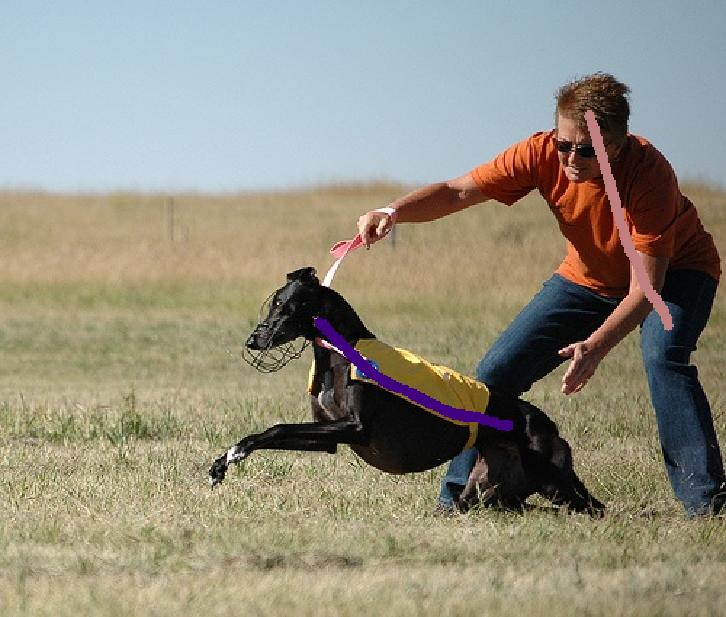
\includegraphics[width=0.24\linewidth]{./draw_and_tell/fig3/006488-scribbles1.jpg} &
\hspace{-4mm} 
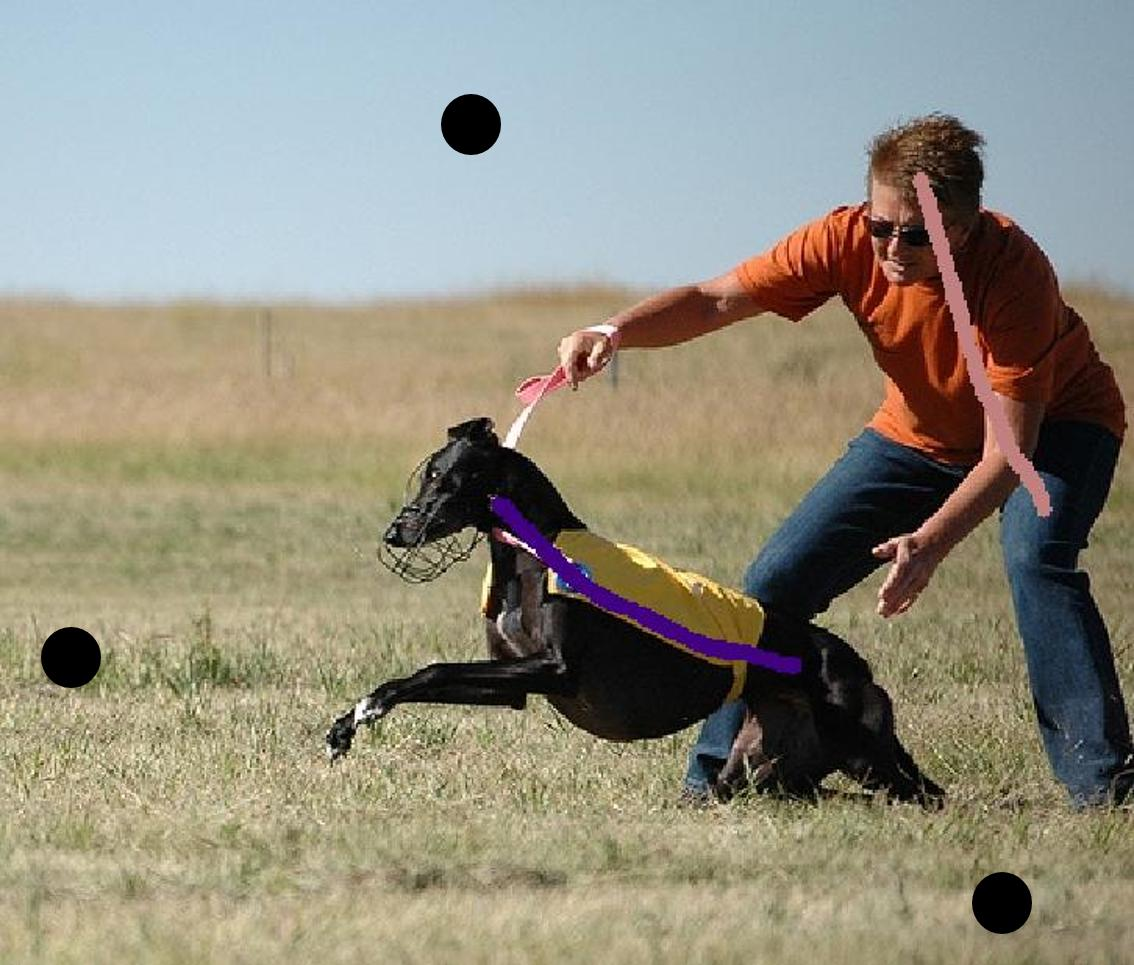
\includegraphics[width=0.24\linewidth]{./draw_and_tell/fig3/006488-scribbles-aug.jpg}&
\hspace{-4mm} 
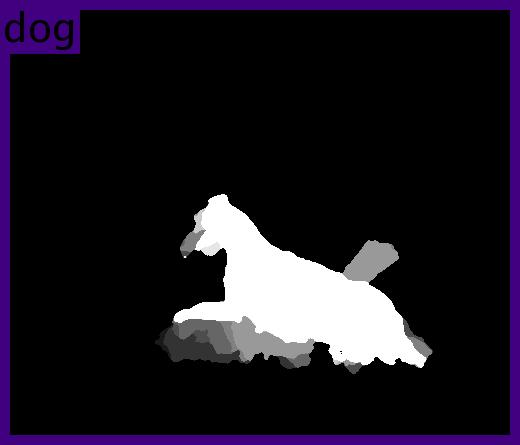
\includegraphics[width=0.24\linewidth]{./draw_and_tell/fig3/heatmap-dog-all.jpg} &
\hspace{-4mm} 
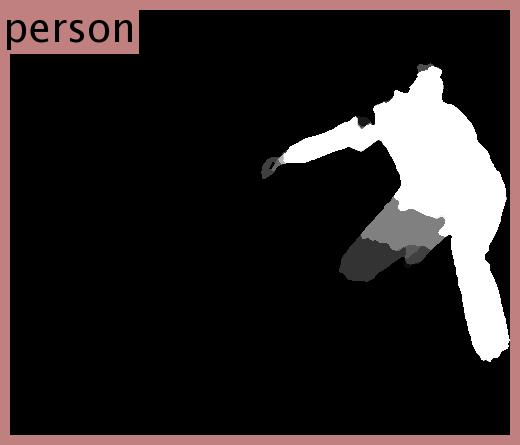
\includegraphics[width=0.24\linewidth]{./draw_and_tell/fig3/heatmap-person-all.jpg} \\

%\hspace{-2mm}
\footnotesize{\text{(a) original scribbles}} & 
%\hspace{-4mm} 
\footnotesize{\text{(b) augmented scribbles}} & 
%\hspace{-4mm}   
\multicolumn{2}{c}{(c) generated semantic heatmaps}  \\
\end{tabular}$
\caption{An example of scribble augmentation and heatmap generation: (a) annotated scribbles; (b) augmented scribbles for the background;
  (c) generated semantic heatmaps for the two objects.}
\label{./draw_and_tell/fig:3}   
\end{figure}

%LUC: FIG.3 TALKS ABOUT THE GEODESIC DISTANCE MAP, BUT THIS COMES OUT OF THE BLUE WHEN FIG.3 IS INITIALLY REFERRED TO. THAT CONCEPT NEEDS SOME  FORM OF EXPLANATION / CONTEXT. 

\subsubsection{Scribble Augmentation}
% \subsubsection{Geodesic distance map}
% We follow the notations used in~\citep{geodesic:star} for geodesic
% distance.

For each class, three (sufficient in practice) more scribbles are
added. For simplicity, they are added sequentially.  New scribbles
should be far from the foreground for good separation, and far from
existing background scribbles to be complementary.  Below, we define
the distance between the scribbles.

%Given two pixels $a$ and $b$ in the image $I$, where $a, b
%\in\{1, ..., W \times H\}$, 
%LUC: NOT SURE WHETHER THAT DEFINITION OF a AND b AS SCALARS IS 
%HELPFUL? IT ACTUALLY SEEMS WRONG FOLLOWING FURTHER DEFINITIONS. 
%I ALSO REFORMULATED SOME OF WHAT FOLLOWS. 
Given an image $I$, all paths that connect pixel $a$ and pixel $b$ are
denoted by $\mathcal{Q}_{ab}$.  Suppose we have a path $\Gamma$
described by the pixels it passes through $\{ \Gamma^1, \Gamma^2,...,
\Gamma^r\}$. The distance between the pixels $\Gamma^1$ and $\Gamma^r$
along path $\Gamma$ is defined as (following~\citep{geodesic:star}):
\begin{equation}
  \label{eq:gdist}
  D(\Gamma) = \sum_{j=1}^{r} \sqrt{ d_{eu}(\Gamma^j, \Gamma^{j+1}) + \lambda \| \triangledown I(\Gamma^j)\|^2}  \enspace ,
\end{equation}
where $d_{eu}(\Gamma^j, \Gamma^{j+1})$ is the Euclidean distance
between two consecutive pixels, and $\| \triangledown I(\Gamma^j)\|^2$
is the gradient magnitude between $(\Gamma^j,\Gamma^{j+1})$, which is
computed by the edge detector of the structured random
forest~\citep{edge:srf}, to avoid texture edges. $\lambda$ is used to
balance the two terms.

Let's denote the existing scribbles as a set of pixels
$\mathcal{E}$. Then, the geodesic distance of pixel $a$ to $\mathcal{E}$ is defined as:
\begin{equation}
  \label{eq:gdist2}
  G(a) =  \min_{b\in \mathcal{E}}  \min_{\Gamma \in \mathcal{Q}_{ab}} D(\Gamma) 
%d_g(a,k) = min
\end{equation}
Without any specific preference, we fix the shape of the new scribble
$\bar{\mathcal{E}}$ to a disk of radius $r=20$ (a balance between
localization and informativeness). Then, the geodesic distance from
the scribble centered at position $a$ to existing scribbles
$\mathcal{E}$ is:
\begin{equation}
  \label{eq:gdist:set}
  G(\bar{\mathcal{E}}_a)  =  \min_{c \in \bar{\mathcal{E}}_a} G(c).
\end{equation}


%LUC: I DON?T UNDERSTAND THIS STORY ABOUT FLAT CIRCLES. IN FIGURE 3
%THE ADDITIONAL SCRIBBLES ON THE BACKGROUND CERTAINLY ARE NO CIRCLES
%AT ALL (THE BLACK ONES). AND WHAT IS THIS `ONE EXAMPLE? IN THE NEXT
%SENTENCE ABOUT? I GUESS YOU WOULD HAVE TO FIX A CIRCLE BEFORE THESE
%DISTANCES CAN BE CALCULATED? WHERE IS THAT CIRCLE CHOSEN IN THE IMAGE
%FOR THIS EXAMPLE? OR IS THIS THE DISTANCE A CALCULATED FOR EACH POINT
%AS CENTER a ? THEN IT IS NOT REALLY ONE EXAMPLE, BUT THE FULL SET OF
%DISTANCES, I.E. FOR ALL POSSIBLE CHOICES OF CENTER a? 

%One example for $G( \bar{\mathcal{E}}_a)$ is shown in
%Figure~\ref{./draw_and_tell/fig:3}(b) for the existing scribbles on the dog and the
%person in Figure~\ref{./draw_and_tell/fig:3}(a).
The sampling probability for the next scribble is then defined as: 
\begin{equation}
  \label{eq:sampling}
  Pr(a) = \frac{\text{exp}(G(\bar{\mathcal{E}}_a)^2 / \sigma^2)} {\sum_{b=1}^{WH} \text{exp} (G(\bar{\mathcal{E}}_b)^2 / \sigma^2)}
\end{equation}
where $\sigma$ is set adaptively to the average of all $G(\bar{\mathcal{E}}_a)$.  
$Pr(a)$ needs to be updated each time a new
scribble is added. One example of $Pr(a)$ for all values of $a$ is shown in Figure \ref{./draw_and_tell/fig:4}. 
The randomness introduced by this sampling allows for the ensemble approach. Note that other information such
as objectness~\citep{edge:box} can be exploited for sampling the background
scribbles. We leave this as future work.

\begin{SCfigure}%{r}{0.5\textwidth}  
%\vspace{-15mm}
$\begin{tabular}{cccccc}
\hspace{-1mm}
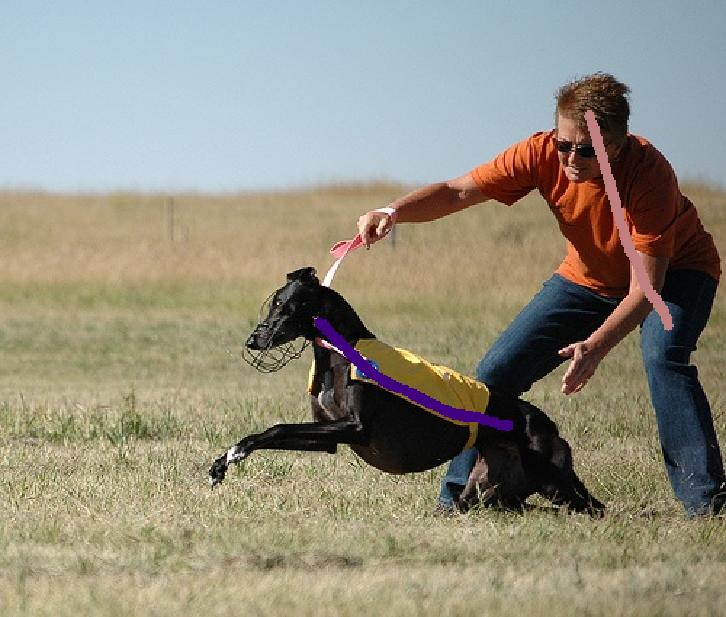
\includegraphics[width=0.3\linewidth]{./draw_and_tell/fig3/006488-scribbles1.jpg} &
\hspace{-2mm} 

\includegraphics[width=0.3\linewidth]{./draw_and_tell/fig3/006488-geodesic.jpg} \\
\hspace{-1mm}
{\text{(a) existing scribbles}} & 
\hspace{-2mm} 
{\text{(b) probability map}} \\ 
\end{tabular}$  %\vspace{-2mm}
\caption{
Probability map for sampling the next new scribble
  (\cf Equation~\ref{eq:sampling}).}
\label{./draw_and_tell/fig:4}  %\vspace{-6mm}
\end{SCfigure}

\subsection{Heatmap-based FCN}

FCN~\citep{Long_2015_CVPR} is designed to regress the 2D label map $O
\in \{1,2,..., K\}^{W \times H}$, directly from the input image $I$.  The output of FCN is 
$K$ score maps $S$, one for one class, i.e. $S \in \mathbb{R}^{W \times 
H \times K}$.  The class labels are obtained either by simply taking the
best-scoring classes at each pixel~\citep{Long_2015_CVPR} or by using
conditional random fields for further refinement~\citep{cnn:em}. FCN 
is trained to minimize the prediction error of cross-entropy over all 
pixels, and its optimization function is:
\begin{equation}
  \label{eq:fcn}
  \mathcal{L} = \sum_{n=1}^N  \sum_{a=1}^{WH}  \mathcal{L}_{na}(S_{na}, O_{na}),
\end{equation}
where $N$ is the number of training images and $\mathcal{L}_{na}$ is
the per-pixel loss function, which is commonly defined as: 
\begin{equation}
  \label{eq:fcnloss}
\mathcal{L}_{na} =  -\text{log} \left( \frac{ \text{exp}(S_{na}^{O_{na}})} {\sum_{k=1}^K \text{exp}(S_{na}^k)} \right).   
\end{equation}
The loss function is only computed for pixels having ground truth
labels. Otherwise, the loss function is set to zero.
 

Directly applying FCN to our training annotations is problematic, as
our annotations are soft semantic heatmaps rather than crisp
segmentation masks. To solve this, we extend the loss function in
Equation~\ref{eq:fcnloss} to the following:

\begin{equation}
  \label{eq:ourloss}
\mathcal{L}_{na}^\prime =  \sum_{k=1}^K P_{na}^k \left[ -\text{log} (\frac{ \text{exp}(S_{na}^k)} {\sum_{k^{\prime}=1}^K \text{exp}(S_{na}^{k^\prime})}) \right].    
\end{equation}
By the adaptation, the loss function is modulated by the heatmaps of
relevant classes -- for each pixel, the most confident classes affect
the loss function the most.  It can be seen that the loss function on
crisp segmentation masks in Equation~\ref{eq:fcnloss} is a special case of
our new loss function. The new loss function can be optimized the same
way as used in standard FCN, with a modification to the loss layer.
We call the model heatmap-based FCN (HFCN), and its pipeline is shown
in Figure~\ref{./draw_and_tell/fig:2}.


\section{Experiments}
\label{drawtell:sec:experiments}
We evaluate HFCN with different settings, and compare it to other
competing methods. The goal is to show that training with
scribbles-based annotations is a good trade-off between annotation
cost and prediction accuracy.

\subsection{Experimental Settings}
\textbf{Dataset}: We evaluate HFCN on PASCAL VOC
2012~\citep{pascal:2011}, which comes with three subsets: training
($1464$ images), validation ($1449$ images) and test ($1456$ images),
having $20$ object classes annotated in full segmentation masks. In
order to keep the same settings with previous
methods~\citep{Long_2015_CVPR, ConsCNN, cnn:em, whatpoint}, we also
extend the training set by adding the extra annotations created by
Hariharan \etal~\citep{semantic:contour} (excluding images from the
original validation set), ending up with $10,582$ training images. The
method is evaluated on the validation set and the test set, under the
metric intersection-over-union (IoU) for all the $20$ classes.

\textbf{CNN}: We adopt the
FCN-8s~\citep{Long_2015_CVPR} model, as it has shown excellent
performance and there is code available. The FCN model is adapted from
the VGG network~\citep{vgg16} pre-trained on the ILSVRC
dataset~\citep{imageNet:challenge}. For the optimization, we employ a
procedure similar to FCN: the SGD solver is used, with an initial
learning rate of $10^{-6}$; the network is trained with $80,000$
iterations.  HFCN is implemented with the Caffe
framework~\citep{Caffe}.% We use a mini-batch of $10$ images.
% Fne-tuning of HFCN on the \emph{train-aug} set of PASCAL VOC 2012
% takes about $30$ hours on a NVIDIA Tesla K40 GPU.

%The parameter $\lambda$ in Equation~\ref{eq:gdist} is set the same way as used in~\citep{geodesic:star}. 

\begin{table*}[tb]
\centering
\scalebox{0.85}{
\setlength\tabcolsep{0.2em} {
  \begin{tabular}{|c|c|c|c|c||ccc|c}   \hline
    Supervision  & Image-level & Point & Bounding-box & Full-mask   &     \multicolumn{3}{c|}{Scribbles (ours)}   \\  \hline 
    Method & ConsCNN  & WhatPoint & CNN-EM  &    FCN-8s  & HFCN-1.5 & HFCN-3  & HFCN-3+CRF   \\   
    mIoU & 35.3 &  42.7     & 60.6 & 62.7  & 56.2 & 61.9 & 64.1 \\  \hline
\end{tabular}}}
\caption{The results of different methods with varying levels of supervision on the validation set of PASCAL VOC 2012.}
\label{table:val} %\vspace{-4mm}
\end{table*}

  % \begin{table}[tb]
 %    \centering
 %    \begin{tabular}{|c|c|c|c|c|c|c|}
 %     Method & Supervision  & val IOU  & test IOU \\ \hline
 % % image-level & point-based & bounding-box & full-mask & ours  \\ \hline
 %      % 32.0        &  42.7   &      
 %    \end{tabular}
 %    \caption{comparison to other methods}
 %  \end{table}
  \begin{table}[tb]
    \centering
%\def\arraystretch{1.2}
\scalebox{0.72}{
\setlength\tabcolsep{0.05em} {
    \begin{tabular}{|cccccccccccccccccccccc|cccccccccc}
      \hline 
     Method & \tvbox{aerop}  & \tvbox{bike}  & \tvbox{bird} & \tvbox{boat} &\tvbox{bottle} &\tvbox{bus}  &\tvbox{car}  &\tvbox{cat}  &\tvbox{chair}  &\tvbox{cow}  &\tvbox{table}  &\tvbox{dog}  &\tvbox{horse}  &\tvbox{mbike}  &\tvbox{person}  &\tvbox{plant}  &\tvbox{sheep}  &\tvbox{sofa}  &\tvbox{train}  &\tvbox{tv}  & mIoU \\ \hline
     
\multicolumn{1}{|l}{\textbf{Image-level}:} &&&&&&&&&&&&&&&&&&&&& \\ 
MIL-FCN & --& --& --& --& --& --& --& --& --& --& --& --& --& --& --& --& --& --& --& --& 24.9  \\   
Img2Pix-CNN & 25.4& 18.2& 22.7& 21.5& 28.6& 39.5& 44.7& 46.6& 11.9& 40.4& 11.8& 45.6& 40.1& 35.5& 35.2& 20.8& 41.7& 17.0& 34.7& 30.4&32.6 \\   \hline
\multicolumn{1}{|l}{\textbf{Single-Point}:} &&&&&&&&&&&&&&&&&&&&& \\ 
What's-point & -- & -- & -- & -- & -- & -- & --& --& --& --& --&-- &-- &-- & --& --& --& --& --&-- & 43.6 \\   \hline

\multicolumn{1}{|l}{\textbf{Bounding-Box}:} &&&&&&&&&&&&&&&&&&&&& \\ 
CNN-EM & 64.4& 27.3& 67.6& 55.1& 64.0& 81.6& 70.5& 76.0& 24.1& 63.8& 58.2& 72.1& 59.8& 73.5& 71.4& 47.4& 76.0& 44.2& 68.9& 50.9& 60.8  \\   
BoxSup & 80.3& 31.3& 82.1& 47.4& 62.6& 75.4& 75.0& 74.5& 24.5& 68.3& 56.4& 73.7& 69.4& 72.5& 75.1& 47.4& 70.8& 45.7& 71.1& 58.8& 64.6  \\   \hline
\multicolumn{1}{|l}{\textbf{Full-mask}:} &&&&&&&&&&&&&&&&&&&&& \\ 
SDS                        & 63.3& 25.7& 63.0& 39.8& 59.2& 70.9& 61.4& 54.9& 16.8& 45.0& 48.2& 50.5& 51.0& 57.7& 63.3& 31.8& 58.7& 31.2& 55.7& 48.5& 51.6 \\   
FCN-8s          & 76.8& 34.2& 68.9& 49.4& 60.3& 75.3& 74.7& 77.6& 21.4& 62.5& 46.8& 71.8& 63.9& 76.5& 73.9& 45.2& 72.4& 37.4& 70.9& 55.1& 62.2 \\   
Zoomout            & 81.9& 35.1& 78.2& 57.4& 56.5& 80.5& 74.0& 79.8& 22.4& 69.6& 53.7& 74.0& 76.0& 76.6& 68.8& 44.3& 70.2& 40.2& 68.9& 55.3& 64.4 \\   
DeepLab-CRF  & 83.5& 36.6& 82.5& 62.3& 66.5& 85.4& 78.5& 83.7& 30.4& 72.9& 60.4& 78.5& 75.5& 82.1& 79.7& 58.2& 82.0& 48.8& 73.7& 63.3& \textbf{70.7} \\   \hline
\multicolumn{1}{|l}{\textbf{Speech-Scribbles}:} &&&&&&&&&&&&&&&&&&&&& \\ 
HFCN-1.5 & 72.1& 32.1& 63.2& 47.0& 59.7& 72.1& 70.4& 72.8& 21.6& 58.2& 41.6& 68.2& 58.2& 71.3& 71.5& 41.4& 56.8& 32.1& 64.5& 52.1&  56.4\\  
HFCN-3     & 76.1& 37.4& 69.3& 53.5& 64.9& 79.6& 74.4& 76.4& 25.9& 62.5& 45.8& 72.3& 62.4& 76.8& 74.6& 45.7& 72.1& 38.3& 68.9& 56.2&  61.7\\  
HFCN-3+CRF & 78.7& 37.5& 71.7& 52.8& 64.5& 78.6& 77.8& 79.7& 25.9& 65.6& 49.9& 75.1& 65.9& 79.4& 76.6& 48.5& 74.9& 39.9& 73.9& 59.5&  63.9\\   \hline      % 32.0        &  42.7   &      
    \end{tabular}  
}}
\caption{Comparison to other methods with different levels of supervision on PASCAL VOC 2012 test.}
\label{table:voc12:test} %\vspace{-6mm}
  \end{table}
  
\subsection{Results}



\textbf{Scribble Augmentation}.  The scribble for the background is
augmented in an ensemble sampling manner, which saves the annotation
cost for the background; background is often large and scattered, so
annotating it can be costly. The parameter $T$ for the ensemble
sampling is evaluated over $10$ values: $[1, 2, ..., 10]$ for HFCN-3.
The results is shown in Fig~\ref{./draw_and_tell/fig:scribble:aug}. As
the figure shows, the performance increases with $T$ from the
beginning and then starts stabilizing.  The scribble augmentation from
each single round has its own weakness and the combination of multiple
rounds `cancels out' the weaknesses because the weaknesses from
different rounds are different due to the randomness in the
sampling. This property has been widely explored in the filed of
ensemble learning. We use $T=10$ for all the following experiments.

\begin{wrapfigure}{r}{0.45\textwidth}  
\vspace{-4mm}
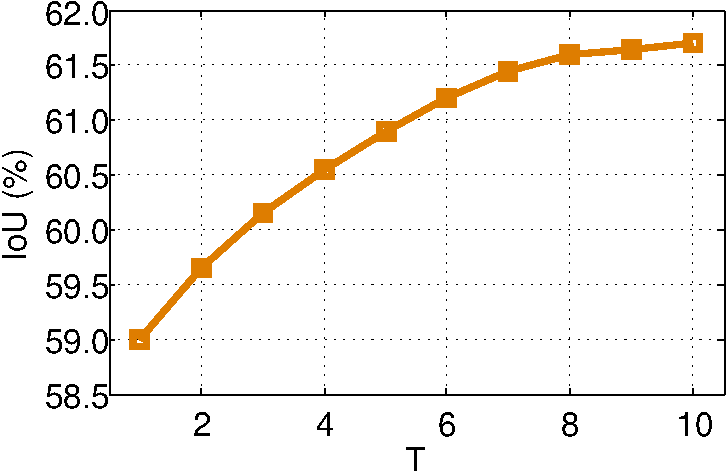
\includegraphics[width=0.95\linewidth,
height=0.65\linewidth]{./draw_and_tell/fig7/scribble_aug_curve.pdf}
\vspace{-3mm}
  \caption{The performance of HFCN-3 as a function of $T$.}
\label{./draw_and_tell/fig:scribble:aug} % \vspace{-6mm}
\end{wrapfigure}



\textbf{Validation Result}: We first evaluate the method on the
validation set.  Table~\ref{table:val} show the results, where the
results of several other methods are also reported for comparison. For
HFCN, we trained it with the two versions of annotations: scribbles
from Anno-1.5 and Anno-3.  They are referred hereafter by HFCN-1.5 and
HFCN-3.  Following the literature~\citep{rcnn_crf,ConsCNN}, we also
added the refinement by CRF~\citep{fully-crf} to Anno-3, which is
referred by HFCN-3+CRF.  It generally true from the table that
stronger (more expensive) supervision leads to better
performance. However, it also shows that with the scribbles by
Anno-1.5, HFCN is already able to yield quite decent results. If the
training data is upgraded to the scribbles of Anno-3, the results are
comparable to that of FCN-8s~\citep{Long_2015_CVPR} and better than
that of CNN-EM~\citep{cnn:em}, though their training annotations are
much more expensive to obtain (\cf Table~\ref{table:speed}). Our
method also shows significantly better results than the
methods~\citep{whatpoint, ConsCNN} trained with comparable annotation
cost.  HFCN-3+CRF further improves the performance on top of HFCN-3,
showing the benefits of combining graphical model and deep neural
networks.  Figure~\ref{./draw_and_tell/fig:5} shows several segmentation
examples.
% This is mainly because for the same object human tend
% to draw similar scribbles under the constraints imposed by the layout
% of the objects, leading to redundant annotations.


\textbf{Test Results}: We also evaluate HFCN on the test
set. Table~\ref{table:voc12:test} shows all the results. The
conclusions drawn on the validation set hold on the test set as
well. Our method obtains results which are comparable to other methods
trained with more expensive supervision, \ie full masks and bounding
boxes, and are better than methods trained with supervision of
comparable annotation cost. These annotation costs are only computed
on the PASCAL VOC training images, however, some competing methods
also use `extra' supervision. For instance,
Img2Pix-CNN~\citep{img:pix:cnn} learns image prior from another larger
set of images; BoxSup~\citep{BoxSup} uses the MCG object
proposal~\citep{MCG} method, which is trained with full-mask
supervision from the PASCAL VOC dataset.  Also, the bounding boxes
used by the two methods~\citep{cnn:em, BoxSup} are generated from the
labeled full segmentation masks, which may transfer some supervision
from there because the generated bounding boxes are often tighter than
those annotated directly by annotators.
% In
% this work, we stick to only the supervision from our annotations in
% order to better show the potentials. 
The performance of HFCN is improved the same way as other
methods~\citep{rcnn_crf, cnn:em, ConsCNN} by  the
CRF~\citep{fully-crf} for further refinement. 

\begin{figure*}[tb]
\scalebox{1}{
$\begin{tabular}{ccccccc}

\hspace{-2mm} 
\rotatebox{90}{\parbox{2cm}{Image}}
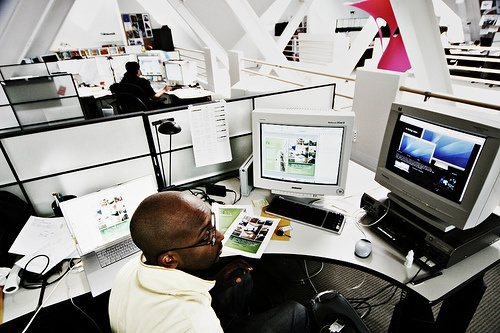
\includegraphics[width=0.23\linewidth, height=0.16\linewidth]{./draw_and_tell/fig5/2007_001678.jpg} &
\hspace{-4mm} 
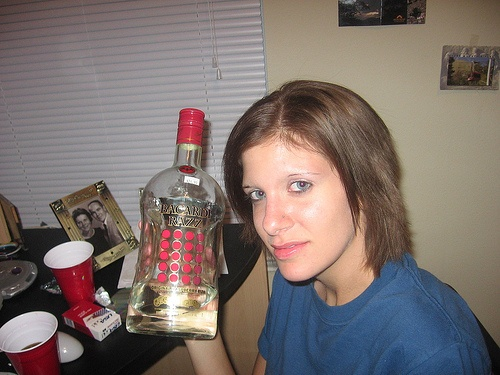
\includegraphics[width=0.23\linewidth, height=0.16\linewidth]{./draw_and_tell/fig5/2007_000346.jpg} &
\hspace{-4mm} 
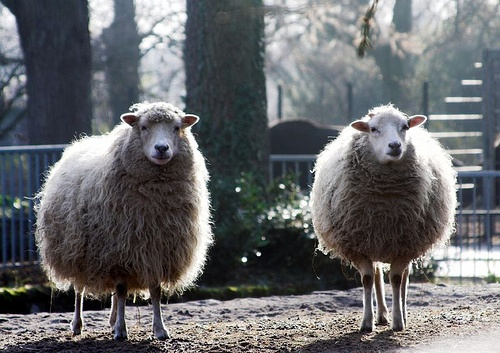
\includegraphics[width=0.23\linewidth, height=0.16\linewidth]{./draw_and_tell/fig5/2007_000925.jpg}  &
\hspace{-4mm} 
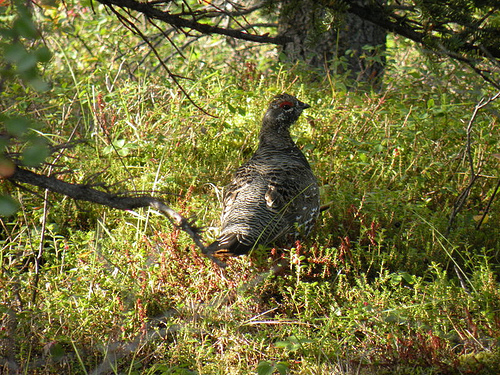
\includegraphics[width=0.23\linewidth, height=0.16\linewidth]{./draw_and_tell/fig5/2009_005260.jpg} \\

\hspace{-2mm} 
\rotatebox{90}{\parbox{2mm}{GT}}
%\footnotesize{\text{GT}}
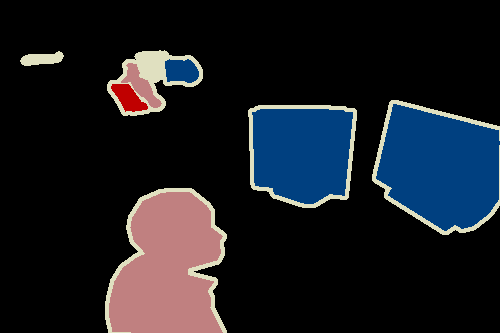
\includegraphics[width=0.23\linewidth, height=0.16\linewidth]{./draw_and_tell/fig5/2007_001678_gt.png} &
\hspace{-4mm} 
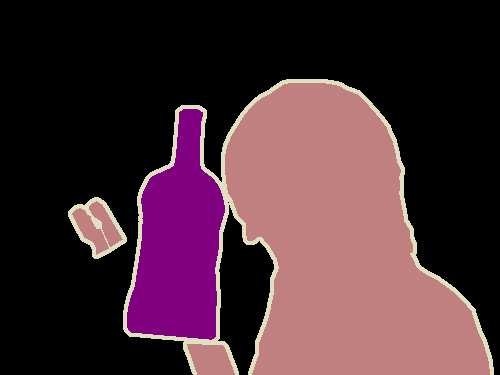
\includegraphics[width=0.23\linewidth, height=0.16\linewidth]{./draw_and_tell/fig5/2007_000346_gt.png} &
\hspace{-4mm} 
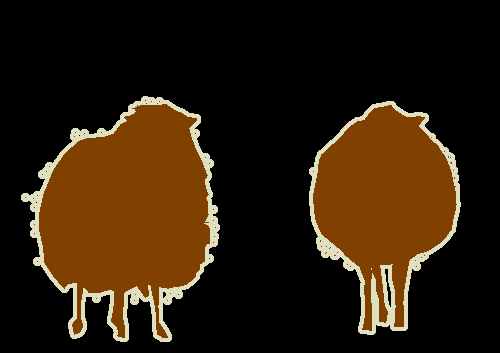
\includegraphics[width=0.23\linewidth, height=0.16\linewidth]{./draw_and_tell/fig5/2007_000925_gt.png} &
%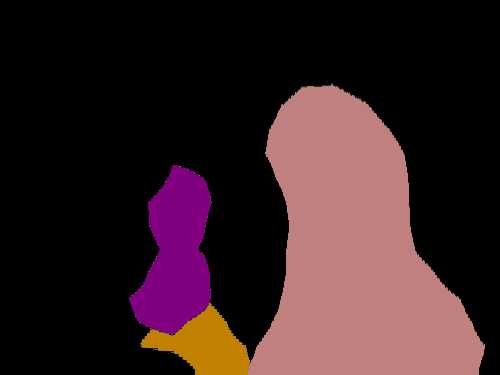
\includegraphics[width=0.24\linewidth]{./draw_and_tell/fig5/2007_000346_res_1.png} &
\hspace{-4mm} 
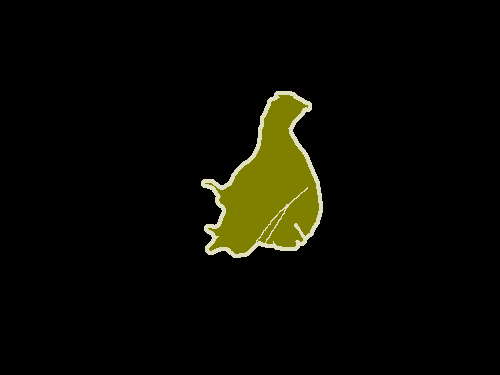
\includegraphics[width=0.23\linewidth, height=0.16\linewidth]{./draw_and_tell/fig5/2009_005260_gt.png} \\

\hspace{-2mm} 
\rotatebox{90}{\parbox{2mm}{Result}}

\includegraphics[width=0.23\linewidth, height=0.16\linewidth]{./draw_and_tell/fig5/2007_001678_res_2.png} &
\hspace{-4mm} 
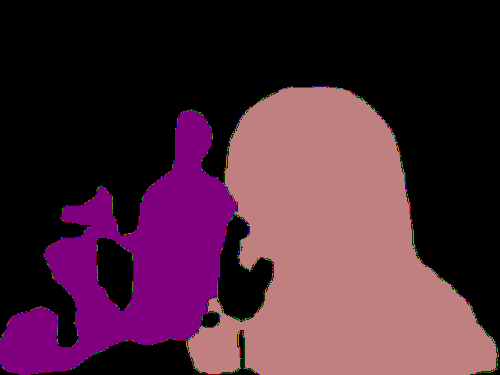
\includegraphics[width=0.23\linewidth, height=0.16\linewidth]{./draw_and_tell/fig5/2007_000346_res_2.png} &
\hspace{-4mm} 
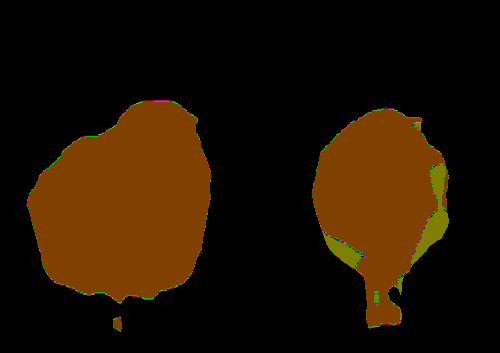
\includegraphics[width=0.23\linewidth, height=0.16\linewidth]{./draw_and_tell/fig5/2007_000925_res_2.png} &
\hspace{-4mm} 
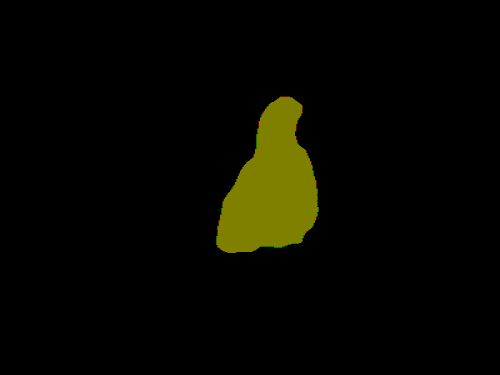
\includegraphics[width=0.23\linewidth, height=0.16\linewidth]{./draw_and_tell/fig5/2009_005260_res_2.png} \\

% \hspace{-1mm}
% \footnotesize{\text{(a) input image}} & 
% \hspace{-1.5mm} 
% \footnotesize{\text{(b) Ground truth}} & 
% %\hspace{-2mm} 
% %\footnotesize{\text{(c) HFCN-1.5 }} & 
% \hspace{-1.5mm} 
% \footnotesize{\text{(d) HFCN-3}} \\ 
 \end{tabular}$}
\caption{Examples of the segmentation results on the validation set of PASCAL VOC 2012.} 
\label{./draw_and_tell/fig:5}
\end{figure*}


\textbf{Annotation Cost vs. Accuracy}: We tabulate the annotation cost
and the mIoU of all the methods considered. See
Figure~\ref{./draw_and_tell/fig:6} for the results. From the plot, it is
evident that HFCN strikes a good balance between annotation speed and
prediction accuracy.  The merit makes our method adaptable and
applicable to new, customized tasks, which is beneficial to many real
vision applications.  As more and more forms of supervision are
explored, we believe that an evaluation of annotation cost
vs. accuracy is very necessary in order to clearly show the trade-offs
made by different alternative approaches.


\textbf{Weak Annotation vs. Strong Annotation}.  The development of
methods with different forms of annotations naturally raises a
question: under a fixed annotation budget, should one work for more
weak annotations or fewer precise annotations?  We answer this
question by comparing the performance of HFCN-3 trained on $9900$
images annotated by Anno-3 to that of FCN-8 trained on $900$ images
with full-mask annotations. The training data for FCN-8 is randomly
sampled from all the training data. $5$ FCN-8 models are trained, each
with its own training set, and their results are averaged. The final
results (mIoU) are: $56.3\%$ for FCN-8 and $60.9\%$ for HFCN-3. The
results are exciting, and they suggest that with the same amount of
annotation effort, our method gathers more semantic information than
the conventional more expensive annotation methods. In a wider
context, the results suggest that gathering weak training data can be
more helpful than gathering strong training data, if the same amount
of annotation effort is given.  Learning with a mixture of strong and
weak annotations can be interesting as well, as shown
in~\citep{BoxSup}. We leave this as our future work.

% \textbf{Training Time}: Another factor that matters is the training
% time. For most of existing methods trained with image-level
% supervision~\citep{img:pix:cnn, cnn:mil} and object
% bounding-boxes~\citep{cnn:em, BoxSup}, an EM-style algorithm is needed,
% meaning that the training (fine-tuning) of CNNs is performed for every
% iteration. This increases the training time. HFCN, however, only needs
% one round of training.

\begin{SCfigure}%{r}{0.5\textwidth}  
  \centering
  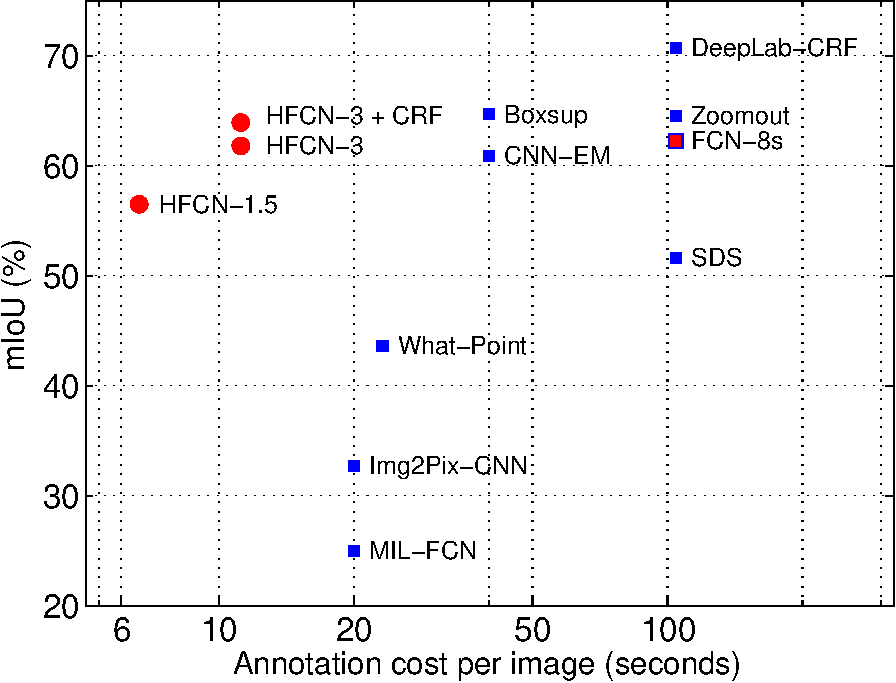
\includegraphics[width=0.65\linewidth]{./draw_and_tell/fig6/anno_cost_mIoU.pdf}  \vspace{-3mm} 
  \caption{Annotation vs. segmentation performance (mIoU) of all the
    methods considered. Evaluated on PASCAL VOC 2012 test.}
\label{./draw_and_tell/fig:6}  
\end{SCfigure}


\textbf{Soft Heatmap vs. Hard Segmentation}. We investigated whether
the soft heatmaps are helpful. To this aim, a baseline is designed for
comparison by simply taking the max object probability from the soft
maps, and then passing the resulting object masks to FCN-8.  We found
that by doing so, the performance drops from $61.7$ to $59.2$. The
advantage of soft heatmaps is that objects (parts) with uncertainties
are left to be decided and explored by the FCN model that has been
trained with objects of higher certainty. The trained FCN model is
more ‘knowledgeable’ than simple thresholding in distinguishing
uncertain objects.


\section{Conclusion}
\label{drawtell:sec:con}
In this work , we developed an annotation method Draw\&Tell to create
training data for semantic image segmentation. Draw\&Tell allows
annotators to simply draw scribbles (strokes) on objects and speak
their names in the meanwhile, solving the \emph{what} and \emph{where}
problems once at the same time. We have proven experimentally that
Draw\&Tell is faster than other annotation methods, \eg $11$ times
faster than full-mask annotation, $4$ times faster than bounding-box
annotations, and $2$ times than the image-level annotation. A method
of integrating visual information and acoustic information is also
proposed for robust object name recognition. This combination can
serve as an example of integrating vision and speech, and inspires
research in this direction. Furthermore, we proposed a method that
allows CNNs models to learn from scribble-based training data, by
converting scribbles to semantic confidence maps and extending
standard CNNs to accommodate soft confidence maps. We showed in
experiments that our annotation method, coupled with the learning
method, yields significantly better results than competing methods
trained with annotations of comparable cost, and yields comparable
results to the methods trained with significantly more expensive
annotations.  Introducing speech recognition to visual annotation is
helpful especially for tasks on mobile devices. This work is just a
very first step in this direction.


